\section{Specification}
The overall specification of the system is described in \cref{intro}.

One of the dangers with a DRSSTC is injury or death by electrocution, the safest and most practical way to prevent this is by a set of procedures regarding operation\todo{Reference procedures}, and the possibility to disconnect the coil rig from the rest of the system easily. To be able to disconnect the coil rig easily a user friendly connector should be used.

A failure mode is the coil rig catching fire due to too much power dissapation, the power limiter should prevent this. Bærebølgedeteksjon, plugging av signalkabel.
\todo{Spesifisere hva som skal være trygt, hvordan kan det være farlig?}

By non-destructive failure propagation we mean that the failure of one module should not propagate to another module. Or lead to the coil rig catching fire or outputting high voltage when it is not expected.

\todo{Overvåkningsfunksjonalitet i systemet}

\todo{Funkjsonelle krav, ikke funksjonelle krav.}



With this specification in mind the system has been partitioned into sub-systems listed below. The sub systems has been assigned an arbitrary part number with the prefix "TK".

\begin{figure}
    \centering
    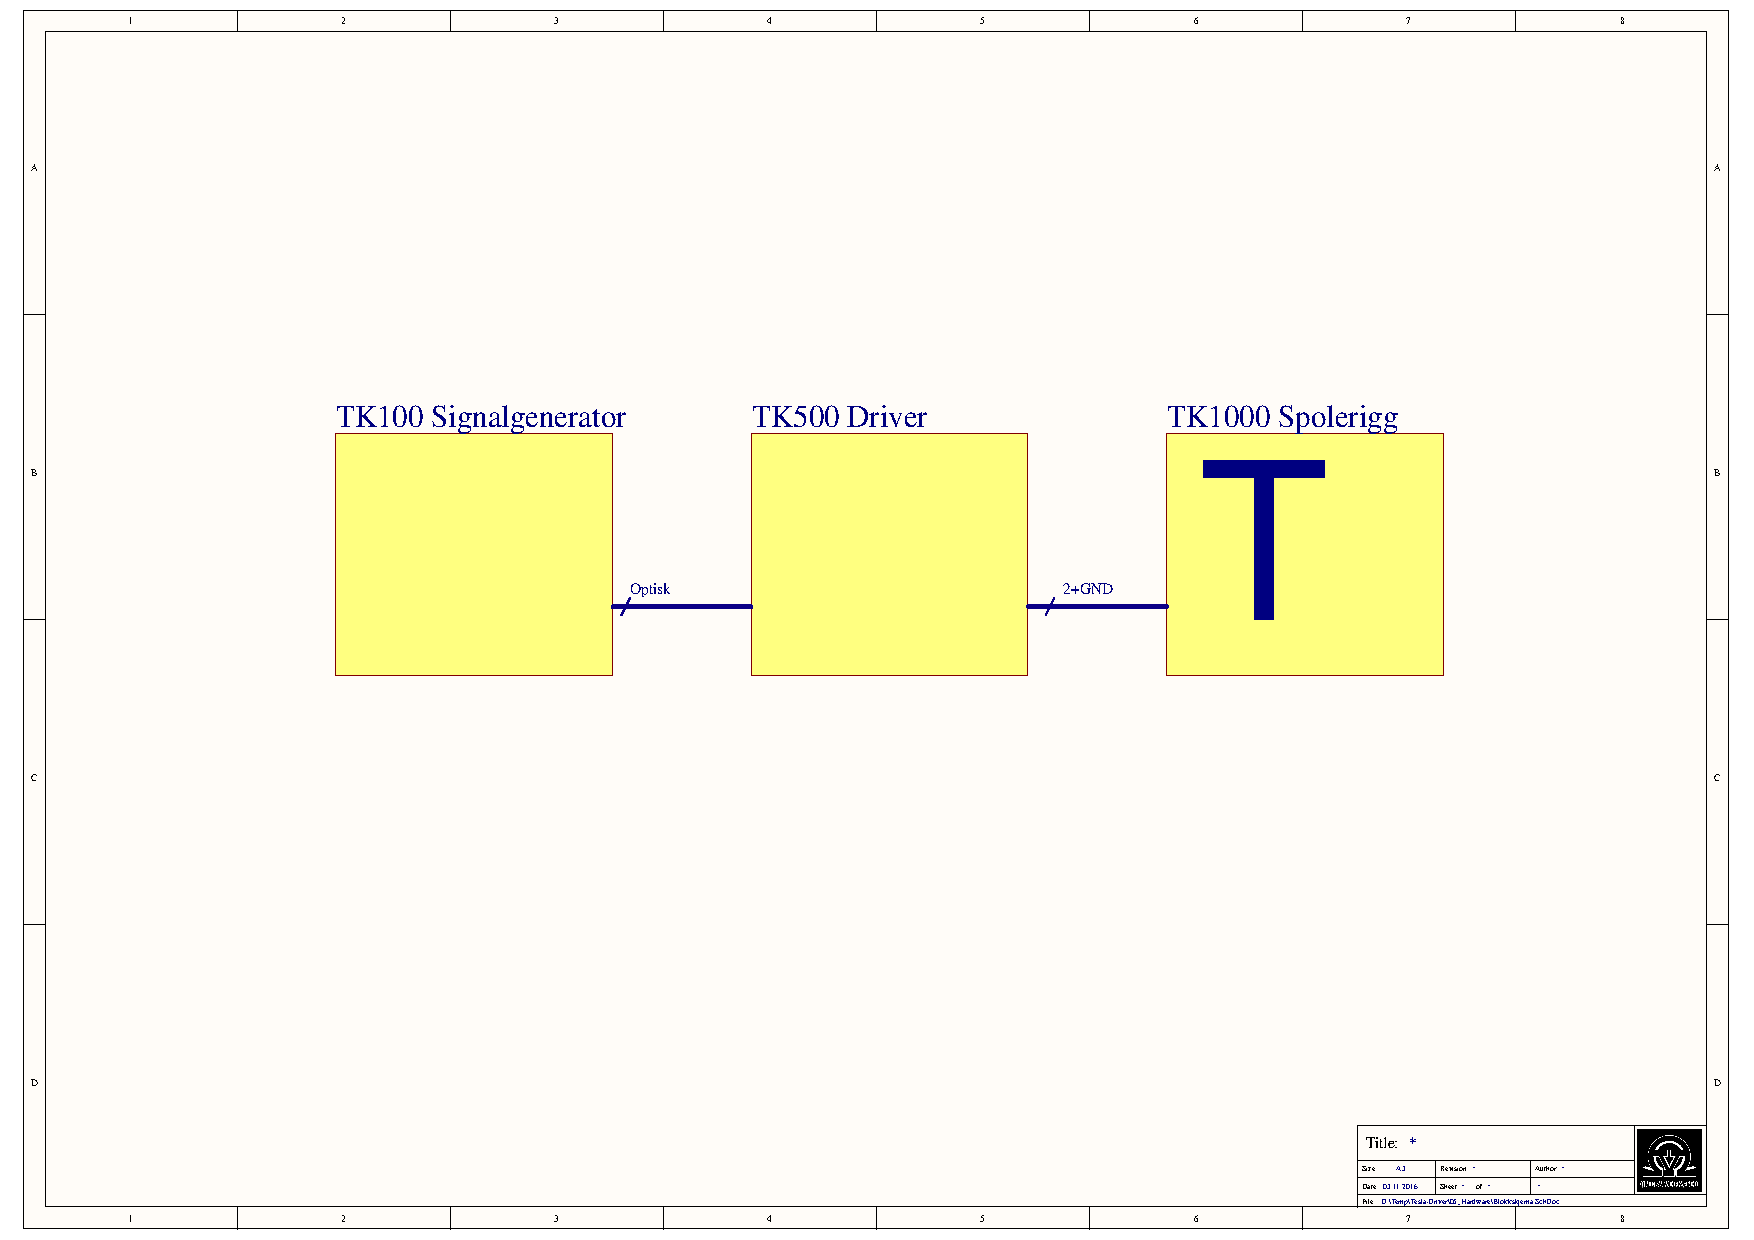
\includegraphics[trim={5cm 9cm 4.8cm 6.5cm},clip,width=\textwidth]{img/Blokkskjema.pdf}
    \caption{Block diagram}
    \label{fig:blokksjema}
\end{figure}

\begin{figure}
    \centering
    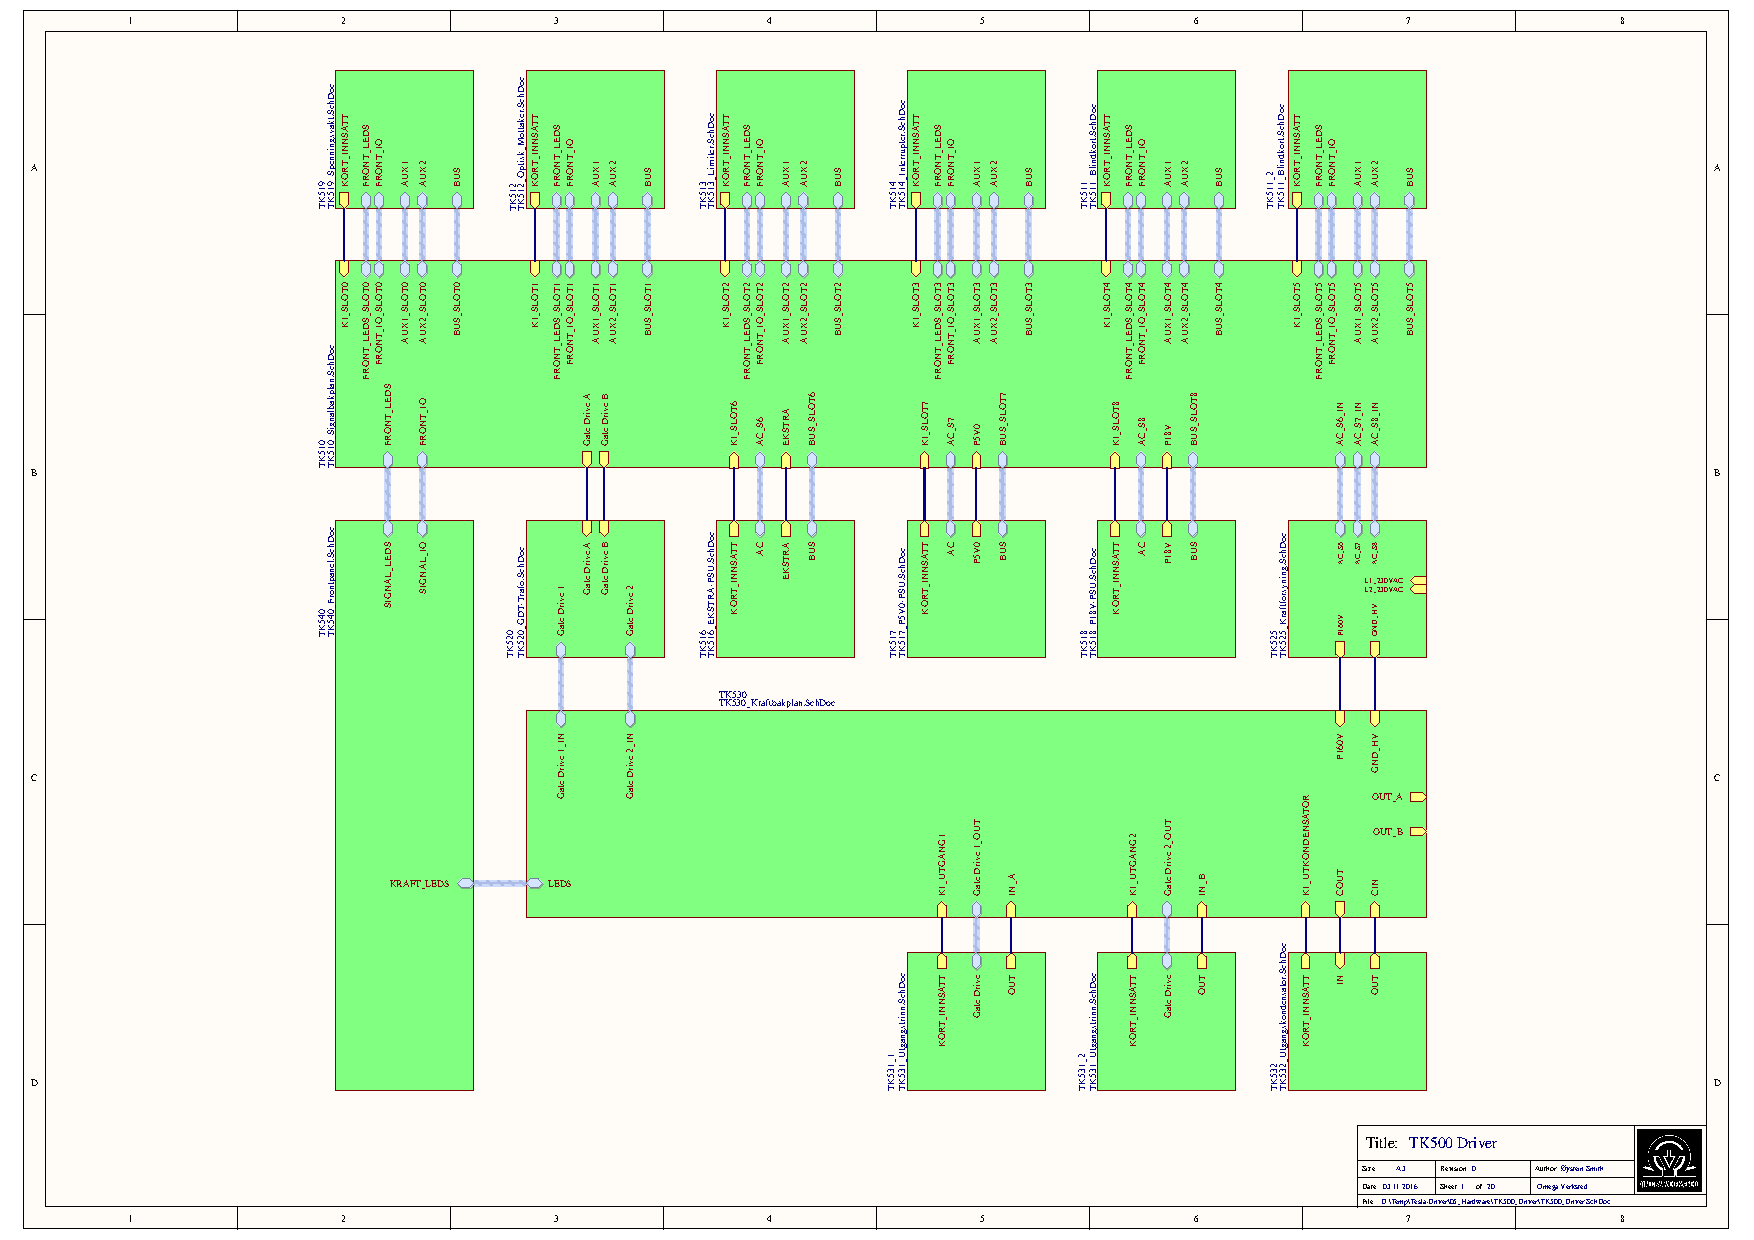
\includegraphics[trim={5cm 2cm 5cm 1cm},clip,width=\textwidth]{img/TK500_Driver.pdf}
    \caption{Block diagram of TK500 Driver}
    \label{fig:tk500}
\end{figure}

\begin{enumerate}
    \item TK100 Signalgenerator
    \item TK500 Driver
    \begin{enumerate}
        \item TK501 Frontpanel
        \item TK502 Frontpanel LEDS
        \item TK510 Signalbakplan
        \item TK511 Blindkort
        \item TK512 Optisk Mottaker
        \item TK513 Limiter
        \item TK514 Interrupter
        \item TK516 Ekstra-PSU
        \item TK517 P5V0-PSU
        \item TK518 P18V-PSU
        \item TK519 Spenningsvakt
        \item TK520 GDT-Trafo
        \item TK530 Kraftbakplan
        \item TK531 Utgangstrinn
        \item TK532 Kondensatorkort
    \end{enumerate}
    \item TK1000 Spolerigg
\end{enumerate}

\subsection{TK100 Signal generator}
The Signal generator Should take a wide range of inputs and output the triggering signal X2 for the driver. It consists of the pulse shaper and signal source mentioned in \cref{DRSSTC} and shown in \cref{fig:func_block}. The output signal X2 should be sent through a optical plastic fibre to be against EMI as mentioned in \cref{sa} and \cref{optical}. The output signal should also be modulated on a carrier wave as described closer in \cref{triggering_signal} and \cref{carrier_wave}.
\todo{Navn på signaler her og i arkitekturseksjonen må stemme med hverandre}

\subsubsection{Triggering signal}
\label{triggering_signal}
The triggering signal X2 should be in the hearable frequency range with a configurable maximal pulse width (high) in the approximate range $0\mu$s - $800\mu$s. The triggering signal should also have a configurable minimum time between pulses.
\subsubsection{Carrier wave}
\label{carrier_wave}
The carrier wave CW for the optical channel should have a sufficiently high frequency $f=\frac{1}{T}$ to transfer the triggering signal X2, in addition to be easily detected in the receivinvg end.\todo{Reference figure in section about optical channel} X2 contains two parts of information the positive flank determining when the tesla coil fires. and the duration of the positive pulse determining the power output (volume). The period $T$ should be shorter than the lowest desirable positive pulse on X2 $T_{X2min}$. \todo{Double check value from experiment} $f_{CW} > \frac{1}{T_{X2min}}$
The shortest desirable pulse on X2 is a length that allows turning the volume down without a noticeable step before shutoff.

\subsubsection{Modulation}
\label{modulation}
The triggering signal should be pulse width modulated PWM with a logical high having a duty cycle of 80\% and logical low having a duty cycle of 20\%.
\begin{figure}[h!]
    \centering
    \begin{tikztimingtable}
        CW (2MHz) & L 17{2C} G 1L \\
        Triggering Signal $X2$ & 9L 8H 19L \\
        PWM & 1L 1H 3L 1H 3L 3H 1L 3H 1L 1H 3L 1H 3L 1L 1H 3L 1H 3L 1L 1H \\
    \end{tikztimingtable}
    \caption{Modulated signal timing diagram}
    \label{fig:cs_td}
\end{figure}{}

\subsection{TK500 Driver}

The driver should take the output of the signal generator (TK100) as input, and output a 160VDC signal at the resonant frequency of the coil rig while the input signal is high and the peak power output does not exceed a configurable level. The driver should also have the capacitor of the primary resonant circuit integrated.

\subsubsection{TK501 Frontpanel}
Should have a height of 4 standard rack units (4U) (17.78cm). Partitioned into multiple parts.
\subsubsection*{Signal back plane card matrix}
Use the entire height, height divided into equal parts for each card in the signal back plane card. Each division should contain four LEDs; Green (Card inserted), Red (Fault), Green (status), Yellow (led in button). A field for card name. Space for buttons depending on the needs of the specific card.

\subsubsection*{Power back plane card matrix}
Three leds for each of the three cards in the power back plane. Green (card inserted), Red (fault), Green (status).

\subsubsection*{Display}
Voltage meter for output voltage.
Ampere meter for output current.

\subsubsection*{Power buttons}
Emergency stop
Spring loaded rotary switch: slow start
Momentary switch: Power on
Momentary switch: Power off

\subsection{TK510 Signalbakplan}
The signal back plane should have six slots for signal modules, and three slots for power supplies.

\subsubsection{Signal module slot}
The signal module slot should have the following signals:
\begin{itemize}
    \item 1 bus with straps for pull up and pull down on bus lines. (B1-B14)
    \item Card inserted detection (A1)
    \item LED signals to front panel (A1-A5)
    \item Misc signals to front panel (A6-A10)
    \item Two contacts for signals other places inside chassis (A11-A14)
    \item Supply voltages and ground (A15-A18 \& B15-B18)
\end{itemize}
The pinout on the module slot connector is shown in \cref{fig:signalmodulslot}

\begin{figure}[h]
    \centering
    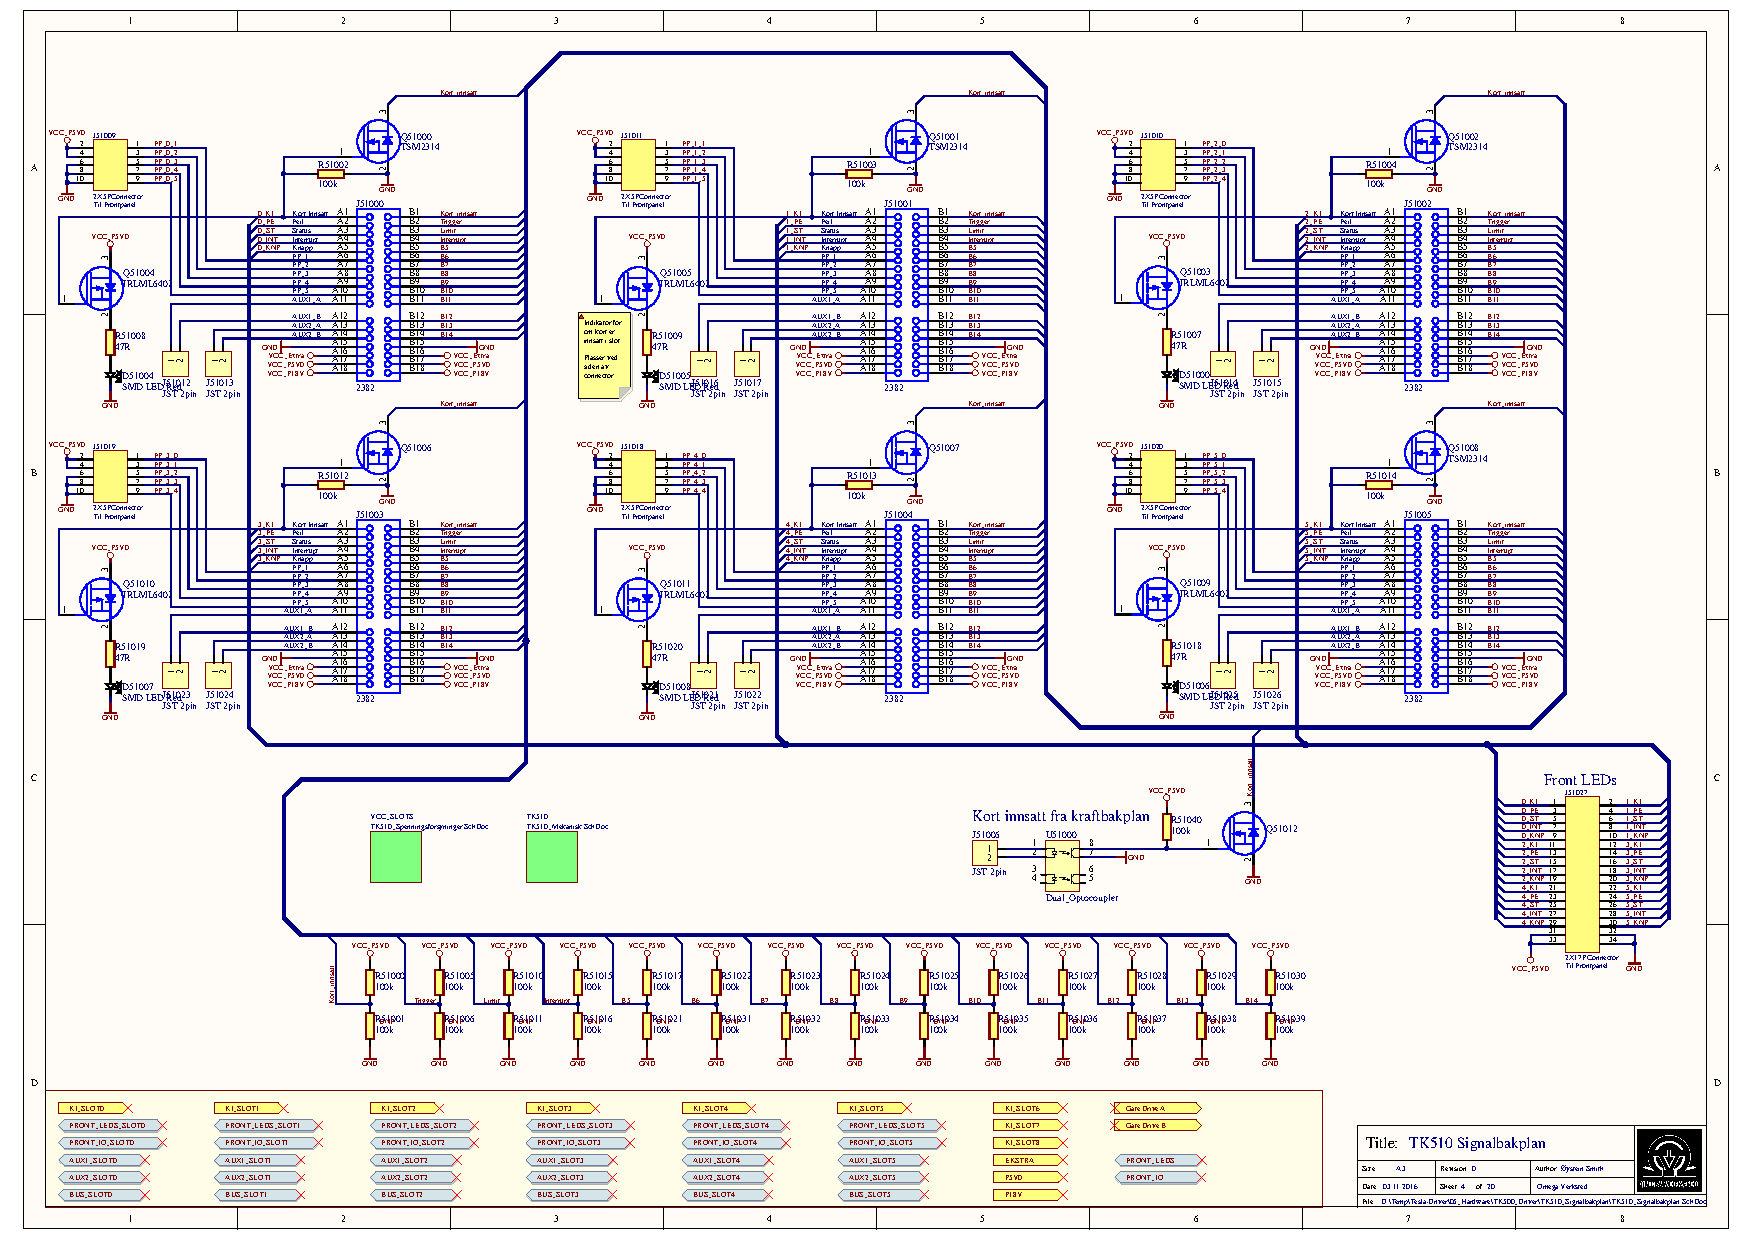
\includegraphics[trim={4.1cm 14.3cm 21.2cm 3.3cm},clip,width=\textwidth]{img/TK510_Signalbakplan.pdf}
    \caption{Signal module card slot connector (detail from schematic of TK510 Signalbakplan)}
    \label{fig:signalmodulslot}
\end{figure}

\subsection{TK511 Blindkort}
The purpose of $TK511$ is to take the space where no module is inserted into the signal back plane, and emulate an inserted module.

\subsection{TK512 Optisk Mottaker}
The purpose of $TK512$ is to convert the optical signal input into the driver $TK500$ to an electrical signal, and a carrier wave detected signal.

\subsection{TK513 Limiter}
The purpose of $TK513$ is to prevent the coil rig $TK1000$ from catching fire, and to keep the spark from turning yellow.

\subsection{TK514 Interrupter}
The purpose of $514$ is to fire the tesla coil when receiving input signal and to tune the output signal via a positive feedback loop to the systems resonance frequency.

\subsection{TK516 Ekstra-PSU}
The purpose of $TK516$ is to reserve a slot for future voltages.

\subsection{TK517 P5V0-PSU}
The purpose of $TK516$ is to provide 5V DC to the driver $TK500$.

\subsection{TK518 P18V-PSU}
The purpose of $TK516$ is to provide 18V DC to the driver $TK500$.

\subsection{TK519 Spenningsvakt}
The purpose of $TK516$ is to monitor the supply voltages in the driver $TK500$.

\subsection{TK520 GDT-Trafo}
The purpose of $TK516$ is to provide galvanic isolation between the signal back plane and the power back plane.

\subsection{TK530 Kraftbakplan}
The purpose of $TK516$ is to provide the connections and monitoring for the output stage $TK531$ and the load capacitor $TK532$.

\subsection{TK531 Utgangstrinn}
The purpose of $TK516$ is to step up the voltage on the output.

\subsection{TK532 Kondensatorkort}
The purpose of $TK516$ is to provide the capacitance of the primary resonance circuit.

\subsection{TK1000 Spolerigg}
The purpose of $TK516$ is to look good and output the voltage arc or corona discharge.